% !TEX encoding = UTF-8 Unicode
\documentclass[10pt]{beamer}

\usepackage{polyglossia}
\usepackage{fontspec}
\usepackage{csquotes}
\usepackage{microtype}
\usepackage{tikz}
\usepackage{color}
\usepackage[backend=biber,style=iso-authoryear,sortlocale=cs_CZ,autolang=other,bibencoding=UTF8]{biblatex}
\usepackage{booktabs}
\usepackage{hyperref}

\usetikzlibrary{decorations.pathreplacing}
\setmainlanguage{czech}
\setmainfont{TeX Gyre Termes}
\usetheme{Boadilla}
\usecolortheme{crane}
\setbeamertemplate{section in toc}[ball unnumbered]
\addbibresource{zotero.bib}

\hypersetup{
	pdfencoding=auto,
	unicode=true,
	citecolor=green,
	filecolor=blue,
	linkcolor=red,
	urlcolor=blue
}

\makeatletter
\newcommand*{\currentSection}{\@currentlabelname}
\makeatother

\newcommand{\mat}{\mathbb}

\title[Hierarchické modely síťového provozu]
{
	Hierarchické modely síťového provozu
}

\titlegraphic
{
	
\includegraphics[width=0.2\columnwidth]{images/fjfi.png}
}

\author[Marek Dědič]
{
	Marek~Dědič\inst{1} \\
	Školitel:~Ing.~Tomáš~Pevný,~Ph.D.\inst{2}
}

\institute[FJFI ČVUT v Praze]
{
	\inst{1} ČVUT v Praze, Fakulta jaderná a fyzikálně inženýrská, Matematická informatika \and
	\inst{2} Cisco Systems Inc., Karlovo náměstí 10, Praha 2
}

\AtBeginSection[]{
	\begin{frame}{\currentSection}
		\tableofcontents[currentsection]
	\end{frame}
}

\begin{document}

\begin{frame}
	\titlepage
\end{frame}

\begin{frame}{Obsah}
	\tableofcontents
\end{frame}

\section{Motivace}
\begin{frame}{Motivace}
	\centering
	\textit{\enquote{100 percent of companies are calling malicious malware hosts}}

	\cite{_cisco_2014}
\end{frame}

\begin{frame}{Data}
	\centering
	\begin{tabular}{lrr}
		\toprule
		\null & \multicolumn{2}{c}{Počet adres} \\
		\cmidrule(l){2-3}
		Datový soubor & Legitimní & Malware \\
		\midrule
		Trénovací legitimní & 417 208 484 & 0 \\
		Trénovací směs & 17 390 889 & 34 359 733 \\
		Testovací legitimní & 1 522 255 052 & 0 \\
		Testovací směs & 2 855 992 & 4 051 944 \\
		\bottomrule
	\end{tabular}
\end{frame}

\section{Řešená úloha}
\begin{frame}{Adresa URL}
	\centering
	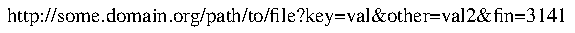
\includegraphics{images/url/url.pdf}
\end{frame}

\begin{frame}{Části adresy URL}
	\centering
	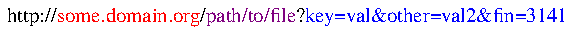
\includegraphics{images/url_parts/url_parts.pdf}
\end{frame}

\begin{frame}{Části a tokeny adresy URL}
	\centering
	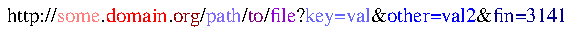
\includegraphics{images/url_subparts/url_subparts.pdf}
\end{frame}

\section{MIL problém}
\begin{frame}{MIL problém}
	\centering
	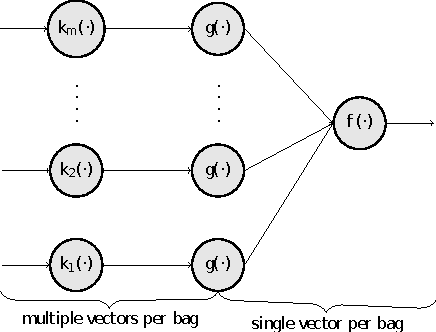
\includegraphics[width=0.7\columnwidth]{images/MIL.pdf}

	\cite{pevny_using_2016}
\end{frame}

\begin{frame}[label=doubleMIL]{Dvojitý MIL problém}
	\centering
	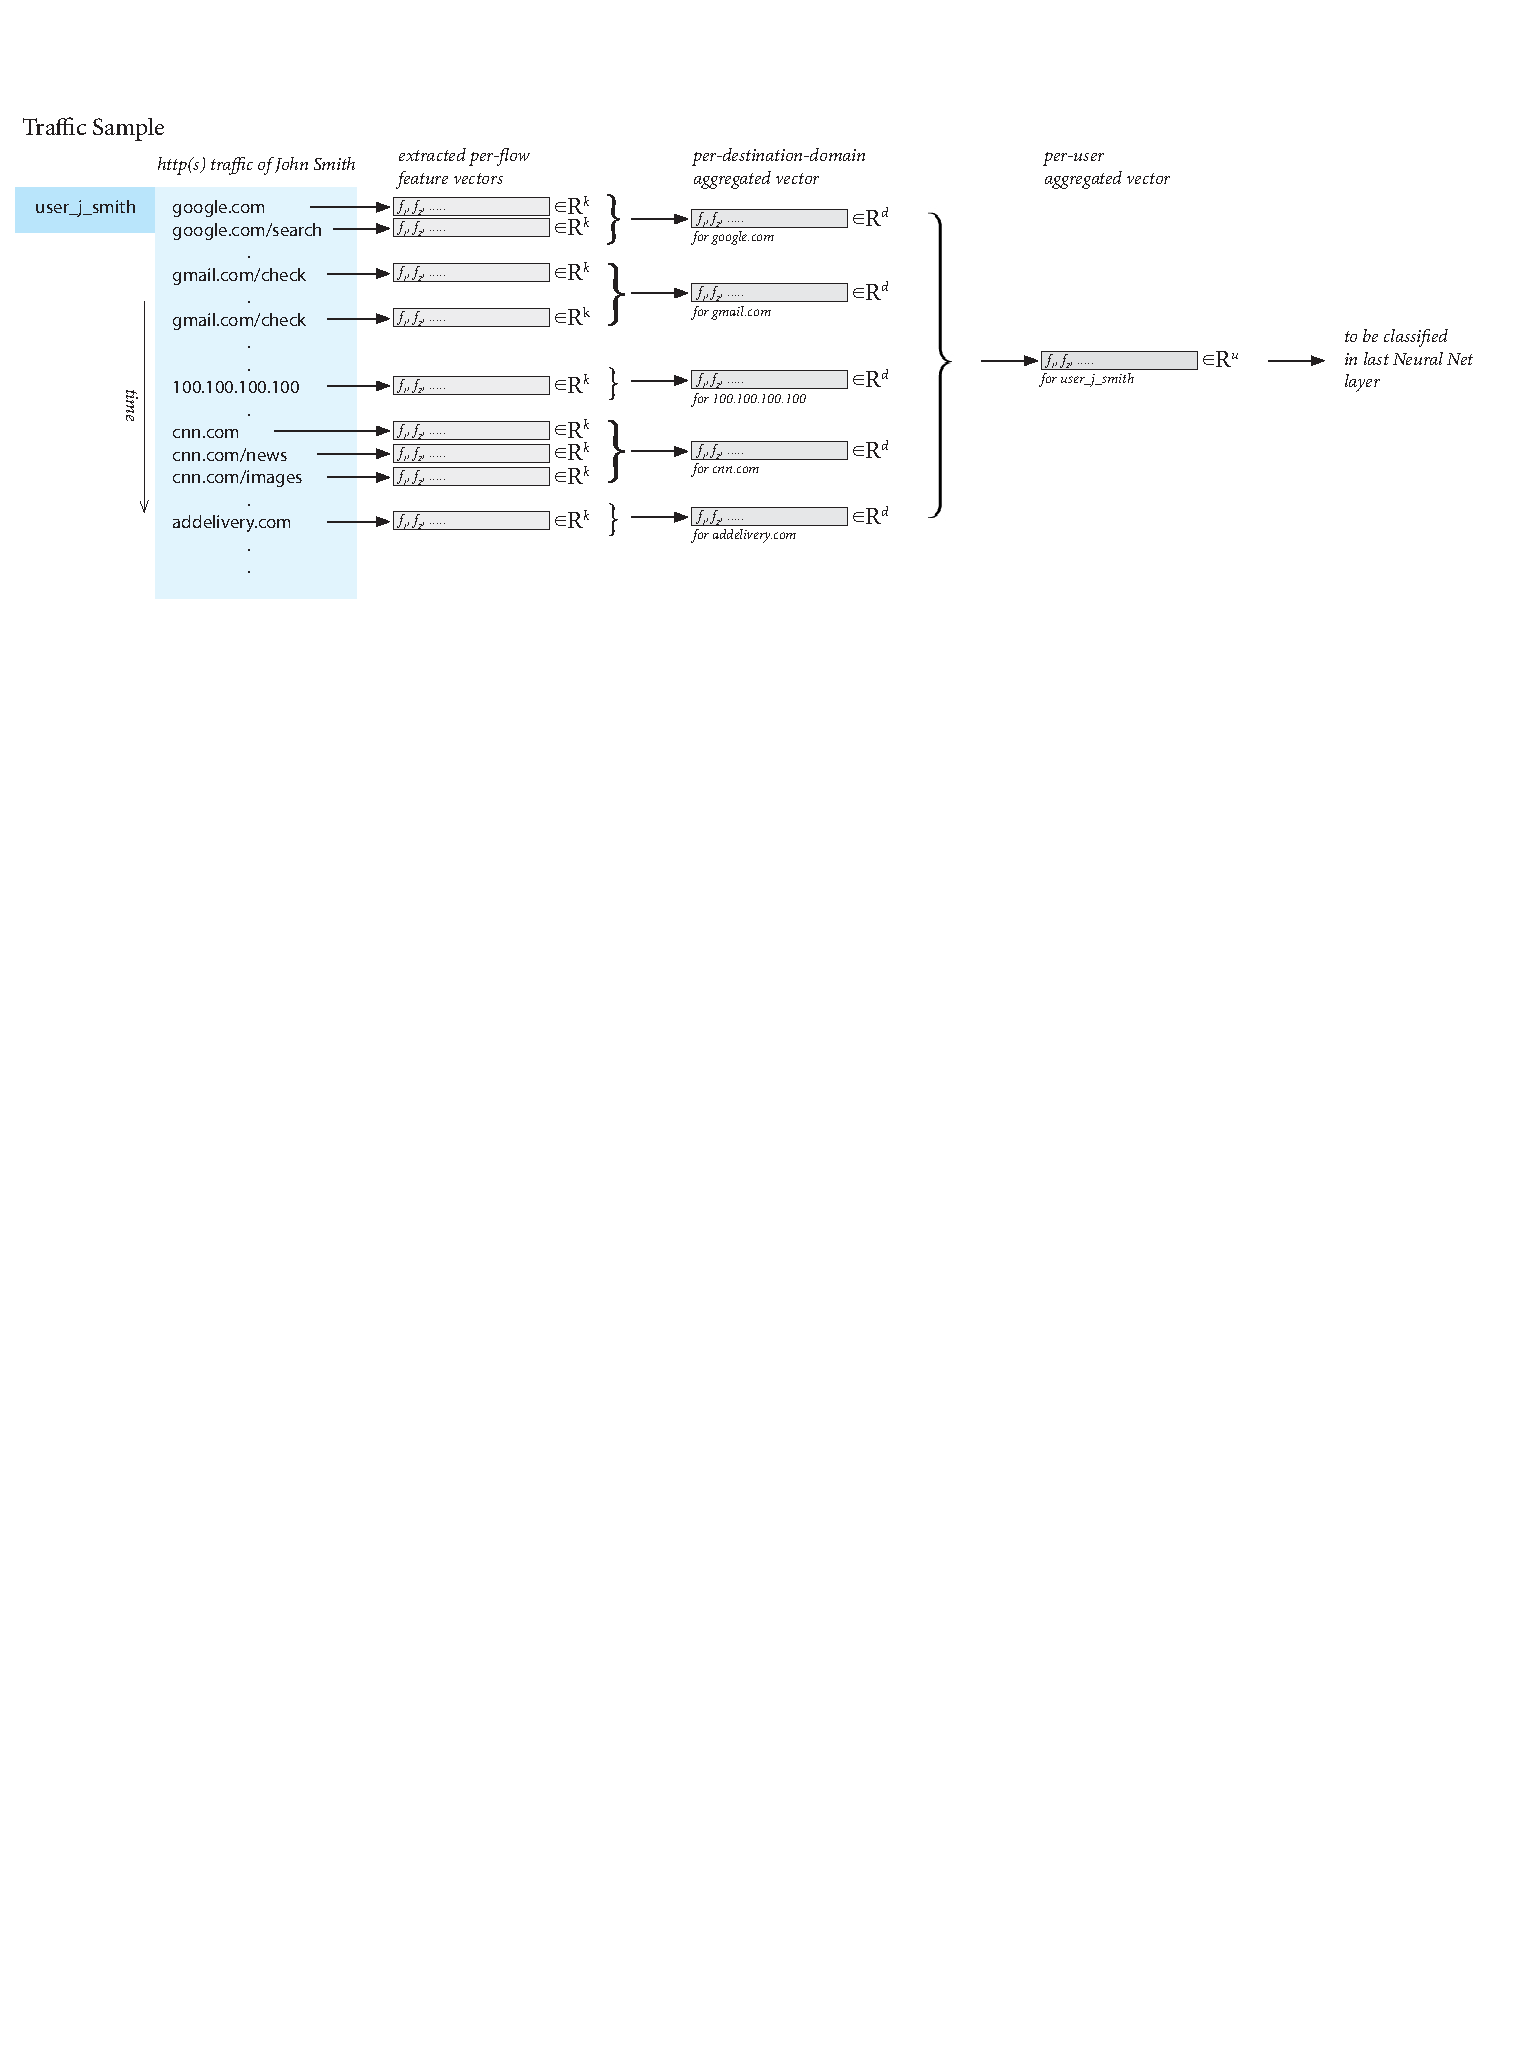
\includegraphics[width=0.9\columnwidth]{images/traffic.pdf}

	\cite{pevny_discriminative_2016}
\end{frame}

\section{Můj přínos}

\begin{frame}{Můj přínos}
	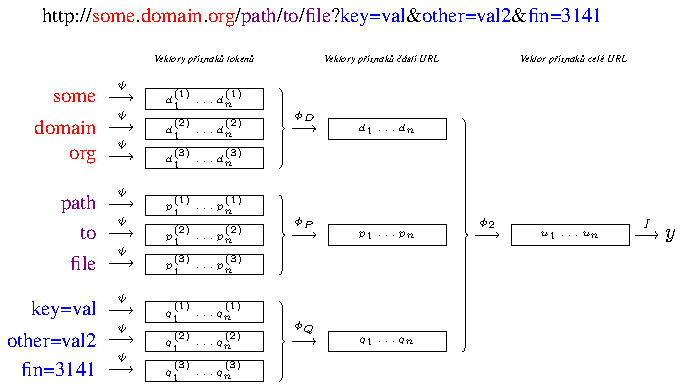
\includegraphics{images/model_modified_MIL/model_modified_MIL.pdf}

	\centering
\end{frame}

\section{Výsledky mé práce}
\begin{frame}{Výsledky mé práce}
	\centering
	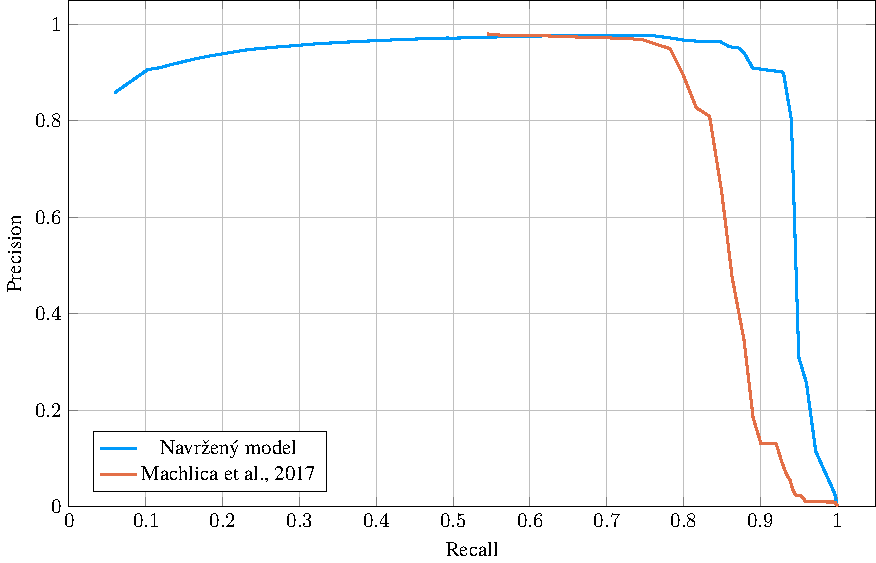
\includegraphics[width=0.9\columnwidth]{images/prior_art/prior_art.pdf}

	Srovnání s \cite{machlica_learning_2017}
\end{frame}

\begin{frame}{Seznam literatury}
	\printbibliography
\end{frame}

\begin{frame}{Hierarchické modely síťového provozu}
	\begin{center}
		\Large{Děkuji za pozornost.}
	\end{center}
\end{frame}

\end{document}
